\subsection{An Example: Donor Spin Coupling}

In order to illustrate the usefulness of the Schrieffer-Wolff transformation, we apply it to the Kane quantum computer~\cite{kane_1998} in order to obtain the effective coupling between phosphorus donor spins.
In this model, each donor spin is coupled to their respective donor electrons via the contact hyperfine interaction.
The two electrons are then coupled to each other via the exchange interaction.
This in turn yields a higher order effectively coupling between the nuclear spins.
The Schrieffer-Wolff transformation then can be used to calculate the form of this interaction.

\begin{figure}[htbp]
    \centering
    % TODO: Add figure. Energy spectrum for Kane QC
    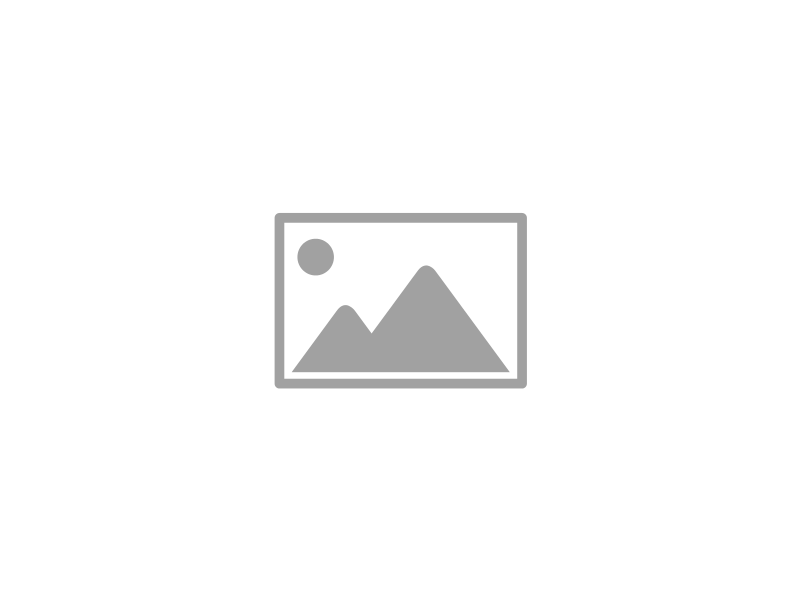
\includegraphics[width=0.75\columnwidth]{placeholder-image}
    \caption[Kane quantum computer energy spectrum.]{The energy spectrum for the Kane quantum computer. Note the well separated energy manifolds. The lowest energy manifold is the one of interest.}
    \label{FIG:kane_qc_spectrum}
\end{figure}

The model can be represented by the Hamiltonian (with $\hbar=1$)
\begin{equation}
    H = -\sum_{i=1,2} \left(\frac{1}{2}\Omega_i \tau_{z}^{(i)} + \frac{1}{2}\omega_i \sigma_z^{(i)} - A_i \vec{\tau}^{(i)}\cdot \vec{\sigma}^{(i)}\right) + J\vec{\sigma}^{(1)}\cdot\vec{\sigma}^{(2)} \,,
\end{equation}
where $\vec{\tau}^{(i)}$ ($\vec{\sigma}^{(i)}$) are the Pauli matrices for the nuclear (electron) spins, $\Omega_i$ ($\omega_{i}$) are the Zeeman energy splittings, $A_i$ are the hyperfine coupling strength for each nuclear-electron spin pair, and $J$ is the electron exchange interaction.
This is a sixteen level system.
However, since the electron Zeeman energy is much greater than the nuclear Zeeman energy, this system is separated into three well-separated energy manifolds corresponding to the three electron spin configurations with different energy (the electron states $\ket{\uparrow\downarrow}$ and $\ket{\downarrow\uparrow}$ have the same energy).
We can then readily see that the hyperfine interactions couple the parallel electron spin manifolds ($\ket{\uparrow\uparrow}$, $\ket{\downarrow\downarrow}$) with the antiparallel manifold ($\ket{\uparrow\downarrow}$, $\ket{\downarrow\uparrow}$) while the exhange interaction couples within the antiparallel manifold.
The Schrieffer-Wolff transformation can be used to reduce this sixteen dimensional system down to a four dimensional system by restricting our space to the two-electron ground state, $\ket{\downarrow\downarrow}$.

We begin the Schrieffer-Wolff transformation by defining our $A$ and $B$ subsets and splitting the total Hamiltonian into the unperturbed Hamiltonian $H_0$ and perturbation $H'$,
\begin{align}
    H_0 & = -\frac{1}{2}\sum_i \left(\Omega_i \tau_{z}^{(i)} + \omega_i \sigma_z^{(i)} \right)                                   \\
    H'  & = \sum_i \left( A_i \vec{\tau}^{(i)}\cdot \vec{\sigma}^{(i)}\right) + J\vec{\sigma}^{(1)}\cdot\vec{\sigma}^{(2)}   \,,
\end{align}
with $A$ being the set of four states in the two-electron ground state and $B$ containing the remaining twelve states.
Following the procedure and equations outlined above up to the third order, we arrive at an effective Hamiltonian,
\begin{multline}
    H_\textrm{eff}= -\frac{1}{2}\sum_i \left( \Omega_i -2 A_i - \frac{4A_i^2(2J+\omega_i-\Omega_i)}{(\omega_i-\Omega_i)^2} \right)\tau_z^{(i)} \\ + 2JA_1A_2\left( \frac{1}{(\omega_1-\Omega_1)(\omega_2-\Omega_1)} + \frac{1}{(\omega_1-\Omega_2)(\omega_2-\Omega_2)}\right)(\tau_x^{(1)}\tau_x^{(2)}+\tau_y^{(1)}\tau_y^{(2)}) \,,
\end{multline}
where the constant term has been omitted.
The Schrieffer-Wolff transformation then allows us to easily see that using the electron exchange and hyperfine interactions as the intermediary between the nuclear spins yields two main effects.
Firstly, the hyperfine interaction introduces a phase shift which is further modified by the exchange coupling.
Secondly, and more importantly, the effective coupling between the nuclear spins is in the form of an $XY$ interaction with strength proportional to $JA_1A_2$ which can be used to build iSWAP gates.